\section{Layer 4: Economy and Micro-Transaction}

\subsection{State Channel Lifecycle}

Nexa-net's state channels provide off-chain, high-frequency micropayment infrastructure between paired agents. A state channel progresses through four lifecycle states:

\begin{figure}[t]
\centering
\begin{tikzpicture}[scale=0.85, every node/.style={font=\small}]
  \node[circle, draw=nexa-green, fill=nexa-green!20, thick, minimum size=1.5cm] (open) at (0,0) {Open};
  \node[circle, draw=nexa-blue, fill=nexa-blue!20, thick, minimum size=1.5cm] (active) at (4,0) {Active};
  \node[circle, draw=nexa-orange, fill=nexa-orange!20, thick, minimum size=1.5cm] (closing) at (8,0) {Closing};
  \node[circle, draw=nexa-red, fill=nexa-red!20, thick, minimum size=1.5cm] (closed) at (12,0) {Closed};

  \draw[->, thick] (open) -- (active) node[midway, above, font=\scriptsize] {deposit locked};
  \draw[->, thick] (active) -- (closing) node[midway, above, font=\scriptsize] {close request};
  \draw[->, thick] (closing) -- (closed) node[midway, above, font=\scriptsize] {settlement};

  \draw[->, dashed, gray] (active) to[loop above] node[font=\scriptsize] {N transfers} (active);
\end{tikzpicture}
\caption{State channel lifecycle: Open $\rightarrow$ Active $\rightarrow$ Closing $\rightarrow$ Closed.}
\label{fig:channel-lifecycle}
\end{figure}

\textbf{Open}: Both parties agree on the initial deposit amounts ($d_A$ from Agent A, $d_B$ from Agent B) and sign a channel opening agreement. The \texttt{ChannelManager} creates the channel with $\text{total\_deposit} = d_A + d_B$ and initializes both balances: $b_A = d_A$, $b_B = d_B$. Channel creation benchmarks at 80.46\textit{ns}.

\textbf{Active}: The channel supports bidirectional transfers. Each transfer adjusts the balance: if Agent A pays Agent B an amount $x$, then $b_A' = b_A - x$ and $b_B' = b_B + x$. A single transfer operation benchmarks at 101.96\textit{ns} (corresponding to approximately 9.9M TPS). The ChannelManager tracks transfer count and cumulative amounts for settlement.

\textbf{Closing}: Either party can initiate a close request. The channel enters the Closing state, after which no further transfers are accepted. The final balances are locked for settlement.

\textbf{Closed}: The SettlementEngine computes the final net balances and records the settlement. The channel resources are released. The balance invariant is verified: $b_A + b_B = \text{total\_deposit}$ must hold at every state transition.

\subsection{MicroReceipt: Dual-Signature and Hash Chain}

Each service call generates a \texttt{MicroReceipt}---a cryptographically signed record of the transaction. The receipt structure contains:

\begin{itemize}
  \item \textbf{payer\_did}: The DID of the paying agent.
  \item \textbf{payee\_did}: The DID of the receiving agent.
  \item \textbf{amount}: The payment amount in NEXA tokens.
  \item \textbf{channel\_id}: The state channel identifier.
  \item \textbf{sequence\_number}: Monotonically increasing counter for ordering.
  \item \textbf{previous\_hash}: SHA-256 hash of the preceding receipt (hash chain link).
  \item \textbf{payer\_signature}: Ed25519 signature by the payer over all receipt fields.
  \item \textbf{payee\_signature}: Ed25519 signature by the payee over all receipt fields + payer signature.
\end{itemize}

The dual-signature mechanism ensures \emph{non-repudiation}: the payer cannot deny making the payment (their signature is on the receipt), and the payee cannot deny receiving it (their signature confirms acceptance). Receipt signing benchmarks at 38.61\textmu s (payer only) and 77.70\textmu s (both signatures). Dual-signature verification benchmarks at 81.24\textmu s, comprising two Ed25519 verification operations plus field validation.

The hash chain links receipts in chronological order: $\text{hash}_i = \text{SHA-256}(\text{receipt}_i)$, and $\text{receipt}_{i+1}.\text{previous\_hash} = \text{hash}_i$. This chain provides: (1) \emph{ordering}: any gap in the sequence indicates missing receipts; (2) \emph{integrity}: modifying any receipt breaks the chain at the next link; (3) \emph{efficiency}: verifying the entire chain requires only checking that each receipt's \texttt{previous\_hash} matches the SHA-256 of its predecessor. Hash computation per receipt benchmarks at 390.93\textit{ns}. Building a 10-receipt chain (including signature + hash linking for each) benchmarks at 17.33\textmu s, approximately 1.73\textmu s per receipt.

\subsection{BudgetController: Multi-Level Budget Enforcement}

The \texttt{BudgetController} implements three levels of budget constraints to prevent resource abuse:

\textbf{Per-call budget}: Each RPC call carries a \texttt{max\_budget} field in the SYN-NEXA message. If the estimated cost (from ACK-SCHEMA) exceeds the per-call budget, the handshake is rejected immediately, preventing wasteful RPC setup.

\textbf{Per-channel budget}: The channel's total deposit limits cumulative spending. Each transfer is validated against the payer's remaining balance: if $b_A - x < 0$, the transfer is rejected. This prevents agents from spending more than they deposited.

\textbf{Per-agent budget}: A global budget cap per agent DID, configurable via \texttt{nexa-proxy.toml}. The BudgetController tracks cumulative spending across all channels for each agent and rejects new channel openings when the agent's total spending exceeds its global budget. This prevents ``spawn many channels'' attacks where an agent opens hundreds of small channels to circumvent per-channel limits.

The three-level budget hierarchy forms a defense-in-depth strategy: the per-call budget prevents single-call overspending; the per-channel budget prevents cumulative overspending within a channel; and the per-agent budget prevents cross-channel overspending by a single agent.

\subsection{SettlementEngine}

When a state channel closes, the SettlementEngine computes the final balances and verifies the balance invariant. The settlement algorithm:

\begin{enumerate}
  \item Collect all MicroReceipts for the channel, ordered by sequence number.
  \item Verify the hash chain integrity: $\text{receipt}_{i+1}.\text{previous\_hash} = \text{SHA-256}(\text{receipt}_i)$ for all $i$.
  \item Verify dual signatures on each receipt.
  \item Compute net transfer amounts: $\text{total\_A\_to\_B} = \sum_{\text{A pays}} \text{amount}$, $\text{total\_B\_to\_A} = \sum_{\text{B pays}} \text{amount}$.
  \item Verify the balance invariant: $b_A' + b_B' = (d_A - \text{total\_A\_to\_B} + \text{total\_B\_to\_A}) + (d_B - \text{total\_B\_to\_A} + \text{total\_A\_to\_B}) = d_A + d_B = \text{total\_deposit}$.
  \item Record the settlement in the global ledger and release channel resources.
\end{enumerate}

If any verification step fails, the settlement enters a \emph{dispute resolution} phase: the last valid receipt in the chain determines the channel state, and all receipts after the break point are discarded. This ``last-known-good'' approach mirrors Bitcoin Lightning's dispute resolution~\cite{lightning2016} but operates on receipt hashes rather than blockchain transactions.

\subsection{Balance Invariant}

The critical safety property of the state channel is the \emph{balance invariant}: at every state transition, the sum of both parties' balances equals the total deposit.

\begin{equation}
b_A(t) + b_B(t) = d_A + d_B = \text{total\_deposit} \quad \forall t
\end{equation}

This invariant is enforced by the channel's transfer logic: each transfer subtracts amount $x$ from the payer's balance and adds the same $x$ to the payee's balance, so the sum is preserved. The invariant is verified: (1) at channel creation (initial state check); (2) after each transfer (balance non-negativity check: $b_A' \geq 0$ and $b_B' \geq 0$); and (3) at settlement (final state verification). Proptest validates this invariant across 1000 random transfer sequences, confirming that no sequence of valid transfers can break the invariant.

\begin{figure}[t]
\centering
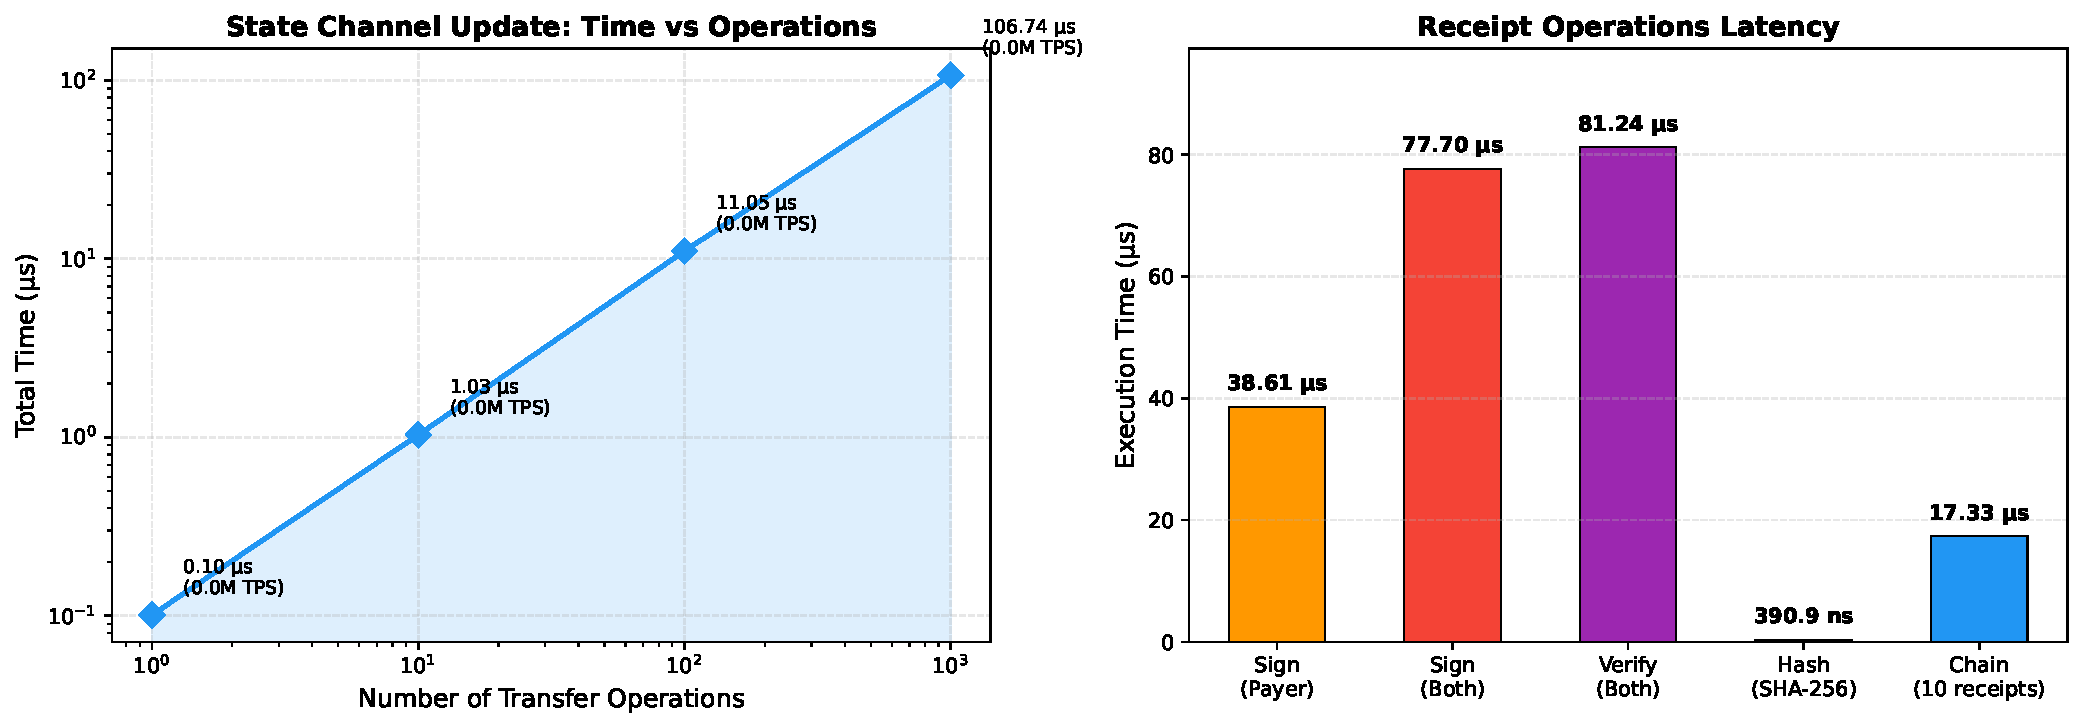
\includegraphics[width=\columnwidth]{figures/economy_bench.pdf}
\caption{Economy layer benchmarks: channel updates at 9.9M TPS (single transfer); receipt signing/verification in 38--81\textmu s range.}
\label{fig:economy-bench}
\end{figure}